\documentclass[a4paper,12pt]{article}
\usepackage[utf8x]{inputenc}
\usepackage[swedish]{babel}
\usepackage[T1]{fontenc}
\usepackage{graphicx}
\usepackage{subcaption}
\usepackage{float}
\usepackage{placeins}
\usepackage{amsfonts, amsmath, amssymb}
\usepackage{ccfonts,euler}
\usepackage{wrapfig}
\usepackage{multirow}
\usepackage{caption}
\usepackage{enumerate}
\usepackage{comment}
\usepackage[includeheadfoot,margin=1.1in]{geometry}
\usepackage{hyperref}
\usepackage{listings}
\usepackage{color}

\definecolor{dkgreen}{rgb}{0,0.6,0}
\definecolor{gray}{rgb}{0.5,0.5,0.5}
\definecolor{mauve}{rgb}{0.58,0,0.82}

\lstset{frame=tb,
  language=Python,
  aboveskip=3mm,
  belowskip=3mm,
  showstringspaces=false,
  columns=flexible,
  basicstyle={\small\ttfamily},
  numbers=none,
  numberstyle=\tiny\color{gray},
  keywordstyle=\color{blue},
  commentstyle=\color{dkgreen},
  stringstyle=\color{mauve},
  escapeinside={\%*}{*)},
  breaklines=true,
  breakatwhitespace=true,
  tabsize=3,
  literate={å}{{\r a}}1 {ö}{{\"o}}1 {ä}{{\"a}}1 {Å}{{\r A}}1 {Ö}{{\"O}}1 {Ä}{{\"A}}1
}

\oddsidemargin -15mm
\evensidemargin -15mm
\marginparwidth 5mm
\topmargin -28mm
\textheight 282mm
\textwidth 190mm
\headheight 4mm
\headsep 4mm

\sloppy

\newcounter{iii}\setcounter{iii}{0}
\def\i{\bigskip\noindent\refstepcounter{iii}\textbf{\arabic{iii}.} }
%\def\iotst#1{\par \smallskip \mbox{}\refstepcounter{iii}\hspace*{#1}\textbf{\arabic{iii}.}}
\newcounter{pun}[iii]
\def\pu{\refstepcounter{pun}{\bf(\alph{pun})}\ }
\def\Pu{\par\noindent\mbox{}\refstepcounter{pun}{\phantom{\textbf{\arabic{iii}.}}\hspace{0.2mm}\bf(\alph{pun})}\ }

\def\ext{\subsection*{Extrauppgifter}}

\title{Programmering, Pepper - Pass 5}
\date{2 augusti}

\makeatletter
\let\newtitle\@title
\let\newdate\@date
\makeatother
\begin{document}

  \renewcommand*\rmdefault{ppl}\normalfont\upshape
\pagestyle{empty}
\large
\section*{\newdate\ \  \newtitle}

\i \textbf{Path sum}

Vi ska nu se på matriser med tal och räkna ut vilken väg som ger den minsta summan då vi går från det övre vänstra hörnet till det nedre högra hörnet genom att bara röra sig ner, upp, vänster eller till höger. I exemplet nedanför ser vi en $5\times5$-matris där den optimala vägen är markerad med rött.

$$
\begin{bmatrix}
\textcolor{red}{131}&673&\textcolor{red}{234}&\textcolor{red}{103}&\textcolor{red}{18}\\
\textcolor{red}{201}&\textcolor{red}{96}&\textcolor{red}{342}&965&\textcolor{red}{150}\\
630&803&746&\textcolor{red}{422}&\textcolor{red}{111}\\
537&699&497&\textcolor{red}{121}&956\\
805&732&524&\textcolor{red}{37}&\textcolor{red}{331}
\end{bmatrix}
$$

\pu Skriv ett program som räknar ut vilken väg som ger den minsta summan i $ 5 \times 5 $ matrisen ovanför från övre vänsta hörnet till nedre högra.

\pu Lös samma problem fast med denna $ 80 \times 80 $ matris: \url{https://projecteuler.net/project/resources/p083_matrix.txt}




\i \textbf{Jan Ersa}

Så här börjar en dikt av Gustaf Fröding:

\textit{Jan Ersa ägde Nackabyn,}

\textit{Per Persa ägde Backabyn}

\textit{i By i Västra Ed.}

\textit{Jan Ersa,}

\textit{Per Persa,}

\textit{de höllo aldrig fred.}

När Jan Ersa och Per Persa, på äldre dagar, flyttade in till staden såg de till att de hamnade så långt från varandra som möjligt. Skriv ett program som läser in information om gatorna i staden och som sedan bestämmer mellan vilka två hus den kortaste vägen är som längst, samt längden av denna väg.


\begin{figure}[H]
\centering
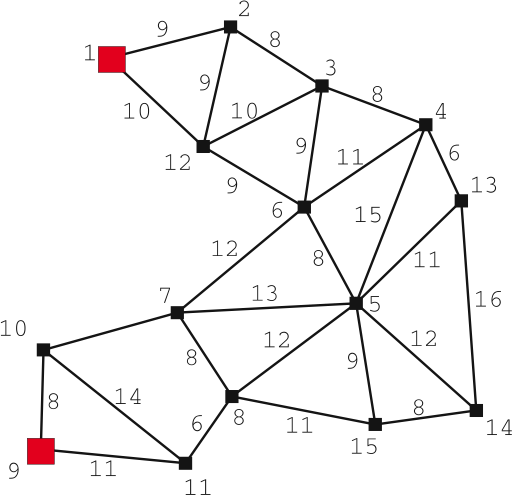
\includegraphics[width=0.4\textwidth]{janErsa}
\caption{Kartan visar stadens alla hus och gator i exemplet. Vi ser också de röda husen där Jan Ersa och Per Persa numera bor. Dessa två hus (nr 1 och 9) är de hus i staden som ligger längst ifrån varandra. }
\label{fig:soldater}
\end{figure}


\textbf{Input:}

På första raden står ett tal $N$
, där $2≤N≤100$, som anger antalet hus i staden. Husen är numrerade från $1$ till $N$. På nästa rad återfinns ett tal som anger antalet gator $V$, där $2≤V≤500$. Därefter följer $V$ rader med tre tal på varje rad: från hus nummer, till hus nummer och gatans längd. Det  går alltid att ta sig från vilket hus som helst till vilket annat hus som helst.

\textbf{Körningsexempel:}
\begin{lstlisting}
Antal hus ? 15
Antal vägar ? 27
1 12 10
1 2 9
2 12 9
6 12 9
3 6 9
2 3 8
3 12 10
3 4 8
4 13 6
5 13 11
5 6 8
4 6 11
4 5 15
6 7 12
7 8 8
8 11 6
9 11 11
9 10 8
7 10 10
10 11 14
8 15 11
5 15 9
5 7 13
5 8 12
5 14 12
13 14 1
14 15 8
Svar: 1 9 49
\end{lstlisting}





\i \textbf{Kinesiska muren}

Den kinesiska kejsaren måste försvara sitt land från de angripande mongolerna. Givet en förenklad karta över det aktuella området (ett $M × N$ rutnät), där vissa rutor är hinder (markerade med ’\#’), bestäm det minsta antal rutor där en mur måste byggas som gör det omöjligt att ta sig från den övre raden i rutnätet (mongolernas område) till den nedersta raden i rutnätet (kinesiskt område). De mongoliska marktrupperna kan bara förflytta sig från en ruta till någon av sina fyra grannrutor om ingen av dessa är hinder eller mur. 

 \textbf{Indata}

Första raden i filen muren.dat innehåller två heltal, $M$ och $N$ $(3 ≤ M,N ≤ 1000)$, storleken på rutnätet. Därefter följer $N$ rader, var och en innehållande M tecken. Varje tecken är antingen ’.’ eller ’x’. Den första och sista raden innehåller enbart ’.’ .

\textbf{Utdata}

Programmet ska först skriva ut en rad med ett tal, det minimala antalet rutor där det måste byggas en mur. Därefter ska det skriva N rader som visar på vilka rutor muren har byggts. Använd samma format som i indatat, men bokstaven ’M’ på de rutor där mur har byggts. Det är tillåtet att bygga mur även på första och sista raden. 


\textbf{Körningsexempel:}
\begin{comment}
Indata:
5 4
.....
..x..
.x..x
.....
Svar:
2
.....
..x..
Mx.Mx
.....
\end{comment}
\begin{lstlisting}
Indata:
12 9
............
....x.......
........x...
.x..x......
.....x......
....x..x...
............
.x....x....x
............
Svar:
6
............
....x.......
........x...
Mx..x......
...M.x......
....xMMxM..
..........M.
.x....x....x
............
\end{lstlisting}



\i \textbf{Brandlarmet:}

Brandlarmet går och du måste ta dig ut så fort som möjligt. Du befinner dig i en byggnad med ett antal utrymmen förbundna med dörrar. Varje utrymme kan klassas som "inomhus" eller "utomhus", och du behöver alltså bara ta dig till ett utrymme som räknas som utomhus. Men vissa dörrar är låsta och nyckeln finns bara i ett visst rum. Det är samma nyckel till alla låsta dörrar.

Det kan alltså ibland vara bättre att först springa och hämta nyckeln så att du sedan kan använda även de låsta dörrarna. Vilket som är det bästa sättet beror förstås på byggnadens utseende. Skriv ett program som, givet en karta över byggnaden, beräknar det minsta antalet sekunder du behöver för att ta dig ut.




\begin{figure}[!ht]
\centering
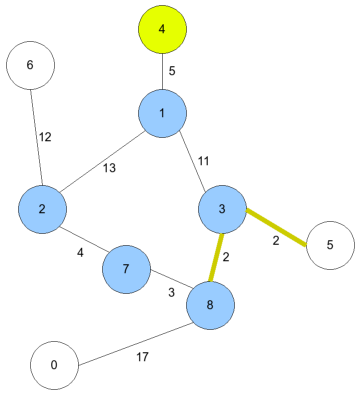
\includegraphics[width=0.4\textwidth]{Brandlarm.png}
\caption{Figuren visar byggnaden i exemplet. Du befinner dig i utrymme 1. De vita ringarna är utomhus, den gula är utrymmet med nyckeln. Talet vid varje förbindelse anger tiden för att springa där, och de gula förbindelserna är låsta. Det snabbaste sättet att ta sig ut är 1 -> 4 -> 1 -> 3 -> 5, vilket tar 5+5+11+2=23 sekunder.  }
\label{fig:brand}
\end{figure}

\textbf{Indata}

På första raden står antalet utrymmen, N, där 1 ≤ N ≤ 2000. Utrymmena är numrerade från 0 till N-1. På den följande raden står två heltal S och Y: numret på utrymmet du befinner dig i från början och numret på utrymmet med nyckeln. Talen uppfyller förstås 0 ≤ S, Y ≤ N-1. Därefter följer N rader med en bokstav på varje rad, antingen i för inomhus eller u för utomhus. Den första raden gäller för utrymme 0, den andra för utrymme 1 o.s.v. Därefter följer ett heltal D, antalet dörrar, där 1 ≤ M ≤ 200000. Slutligen följer M rader med tre heltal P, Q och T och en bokstav (o eller l) på varje rad. Varje rad beskriver en dörr. Talen P och Q är numren på de utrymmen dörren förbinder och T är tiden (i sekunder) det tar att gå igenom dörren. Talen uppfyller 0 ≤ P, Q ≤ N-1 och 1 ≤ T ≤ 1000. Bokstaven betecknar huruvida dören är olåst (o) eller låst (l). Du kan förutsätta att både din startpunkt och nyckeln är inomhus, samt att det alltid finns minst ett sätt att ta sig ut 


\textbf{Utdata}

Programmet ska skriva ut det minsta antalet sekunder som du behöver för att ta dig till ett utrymme som är utomhus. 

\begin{lstlisting}
9
1 4
u
i
i
i
i
u
u
i
i
9
2 1 13 o
3 1 11 o
4 1 5 o
5 3 2 l
6 2 12 o
7 2 4 o
8 3 2 l
8 7 3 o
8 0 17 o

Det krävs åtminstone 25 sekunder
\end{lstlisting}

\end{document}
